\tableofcontents

\chapter{课题背景、意义与国内外研究现状}
\section{研究背景与意义}
近年来,机器人技术飞速发展,机器人已不再局限于在工业领域中完成各种复杂任务,
而是被广泛应用于医疗、教育、军事、交通等各个领域。因此,机器人技术的发展
不仅是未来新兴产业发展的基础、未来科技发展的重要方向之一,也是人类社会发
展的重要组成部分。对于国民经济和国防建设具有重要意义\cite{2013RobotProgress}。

移动机器人分为轮式、履带式和腿足式机器人等。轮式与履带式移动机器人
已被广泛应用于人类社会生活中。但是传统的轮式和履带式机器人由于其地形适应能
力较差,不能适应如楼梯、山地、野外等复杂多变的环境。相比于传统的移动机
器人,腿足式机器人在不同地形上具有更强的适应能力,可以轻松通过崎岖的山路、湿滑的
河滩等复杂地形,成为探险、救援等领域的理想选择\cite{孟健2015复杂地形环境四足机器人运动控制方法研究与实现}。
腿足式机器人又可以细分为双足、四足和六足机器人。双足机器人由于只有两条腿与地
面接触,并且足底与地面支撑面积小,导致其运动灵活性高但稳定性差。
六足机器人由于有六条腿,在运动时可以维持足够大的支撑面积,提高了机器人运动稳定性,
但是腿的数量多也导致其灵活性差\cite{liu2022optimization}。
四足机器人平衡两者的优缺点,展现出更好的稳定性和灵活性。
\begin{figure}[H]
    \centering
    \includegraphics[height=0.3\textwidth]{proposal/spot_mini.png}
    \includegraphics[height=0.3\textwidth]{proposal/ANYmal_arm.png}
    \caption{上图从左到右分别为搭载机械臂的spot mini和ANYmal四足机器人}
    \label{Fig.1.1}
\end{figure}

四足机器人具有很好的运动能力。目前,四足机器人能够穿越各种复杂的地形\cite{hwangbo2019learning, lee2020learning, miki2022learning}。可以替代人
类完成工业巡检,环境检测等任务。尽管四足机器人的
腿足可以充当操作器,去完成推,拉等一些简单的操作任务\cite{arm2024pedipulate, cheng2023legs},
如图\ref{Fig.1.2}所示。
这种方法消弱了原本四足机器人的移动能力,无法让四足机器人在运动过程中同时完成操作任务。
因此,给四足机器人安装机械臂以增加其操作能力是一种直观的想法。通过加装机械臂
,四足机器人不再只是“运动工具”,它变成了具有操作能力的多功能平台。机械臂使得
四足机器人能够执行更为复杂、精细且多样化的任务,极大地扩展了机器人的应用范
围。对于需要跨越不平坦地形、需要高精度操作的任务,加装机械臂的四足机器人展示了
其在多个行业中的潜力,尤其是在救援、物流、农业、制造等领域,它的存在不仅仅是
增强了机器人本身的操作能力,也为未来的智能机器人系统提供了更多的发展可能性,
图\ref{Fig.1.1}展示了搭载机械臂的spot mini和ANYmal四足机器人。
%H为当前位置,!htb为忽略美学标准,htbp为浮动图形
\begin{figure}[H]
    %图片居中
    \centering
    \includegraphics[width=0.86\textwidth]{proposal/pedipulate.png}
    \caption{ANYmal使用腿足充当操作器}
    %用于文内引用的标签
    \label{Fig.1.2}
\end{figure}

在四足机械臂的全身控制系统设计中,机器人的高自由度使得其控制系统设计更加复杂。
目前主流的控制方法是模型预测控制(MPC),该方法能够实现对足式
机械臂的精确控制。然而,MPC方法在实际应用中存在诸多不足,无法避免需要繁琐的建模
过程,并且难以应对高度动态和非结构化的环境\cite{hwangbo2019learning}。相比之下,深度强化学
习(Deep Reinforcement Learning, DRL)近年来在机器人控制领域取得了
显著成果\cite{gu2017deep, kalashnikov2018scalable, chen2023visual},
尤其是在四足机器人运动控制方面展示了强大的适应性和鲁棒性\cite{kim2024not, nahrendra2023dreamwaq}。
DRL是指通过深度学习和强化学习算法来让智能体自主学习并优化决策策略的方法,
该方法无需精确的物理建模,只需通过设计相应的任务奖励函数,通过大规模并行化的
物理仿真实现数据收集,再通过利用强化学习算法就得到高鲁棒性的控制器。
深度强化学习为四足机械臂的全身控
制提供了更加灵活、鲁棒和高效的解决方案,使得机器人可以应对多样化的任务需求和复杂环境。
与MPC相比,DRL减少了繁琐的建模工作,能够让四足机械臂更加智能、自动地适应各种任
务场景,为足式机械臂在各行业的应用带来了更广阔的应用可又能。因此研究基于深度强化学习
的四足机械臂的全身控制方法具有十分重大的意义。
\section{国外研究现状}
关于四足机械臂的全身控制研究,国外起步较早。在2018年,波士顿动力发布了
spot四足机械臂全身协同配合开门的视频。但是波士顿动力从未透露其具体方
法,实现细节无从得知。

2019年,苏黎世联邦理工(ETH)提出了ALMA控制框架\cite{bellicoso2019alma},
这是一个专门为力控四足机械臂设计的运动规划与控制框架,其整体控制框图如图\ref{Fig.1.3}
所示。
该框架已在搭载Kinova机械臂的ANYmal四足机器人上进行验证。
通过使用该控制框架,足式机械臂能够在执行操作任务
的同时保持动态步态运动。此外,它可以使足式机械臂对外部施加的作用力做出顺
应性反应,并在执行运动和操作任务的过程中抵抗扰动以保持平衡。ALMA框架
首先建立了足式机械臂的全身动力学模型。当获得机械臂末端执行器和本体的参考
速度后,在线运动规划器会处理这些速度参考信号,从而生成四足机器人的重心轨
迹和机械臂末端执行器的运动轨迹。接着,通过基于分层优化的全身控制算法进行
跟踪,该算法会生成所有驱动关节的力矩参考信号,从而实现足式机械臂的全身控
制。尽管在该框架中,足式机械臂能够在执行操作任务时展示身体与机械臂之间的
配合动作,但是这种配合动作的实现依赖作者设计的动作映射即机械臂下降时,
四足机器人身体姿态便呈现下伏姿势。这种动作映射无法让机器人依据自身状态产生不同
的配合动作,限制了足式机械臂的应用场景。
\begin{figure}[H]
    %图片居中
    \centering
    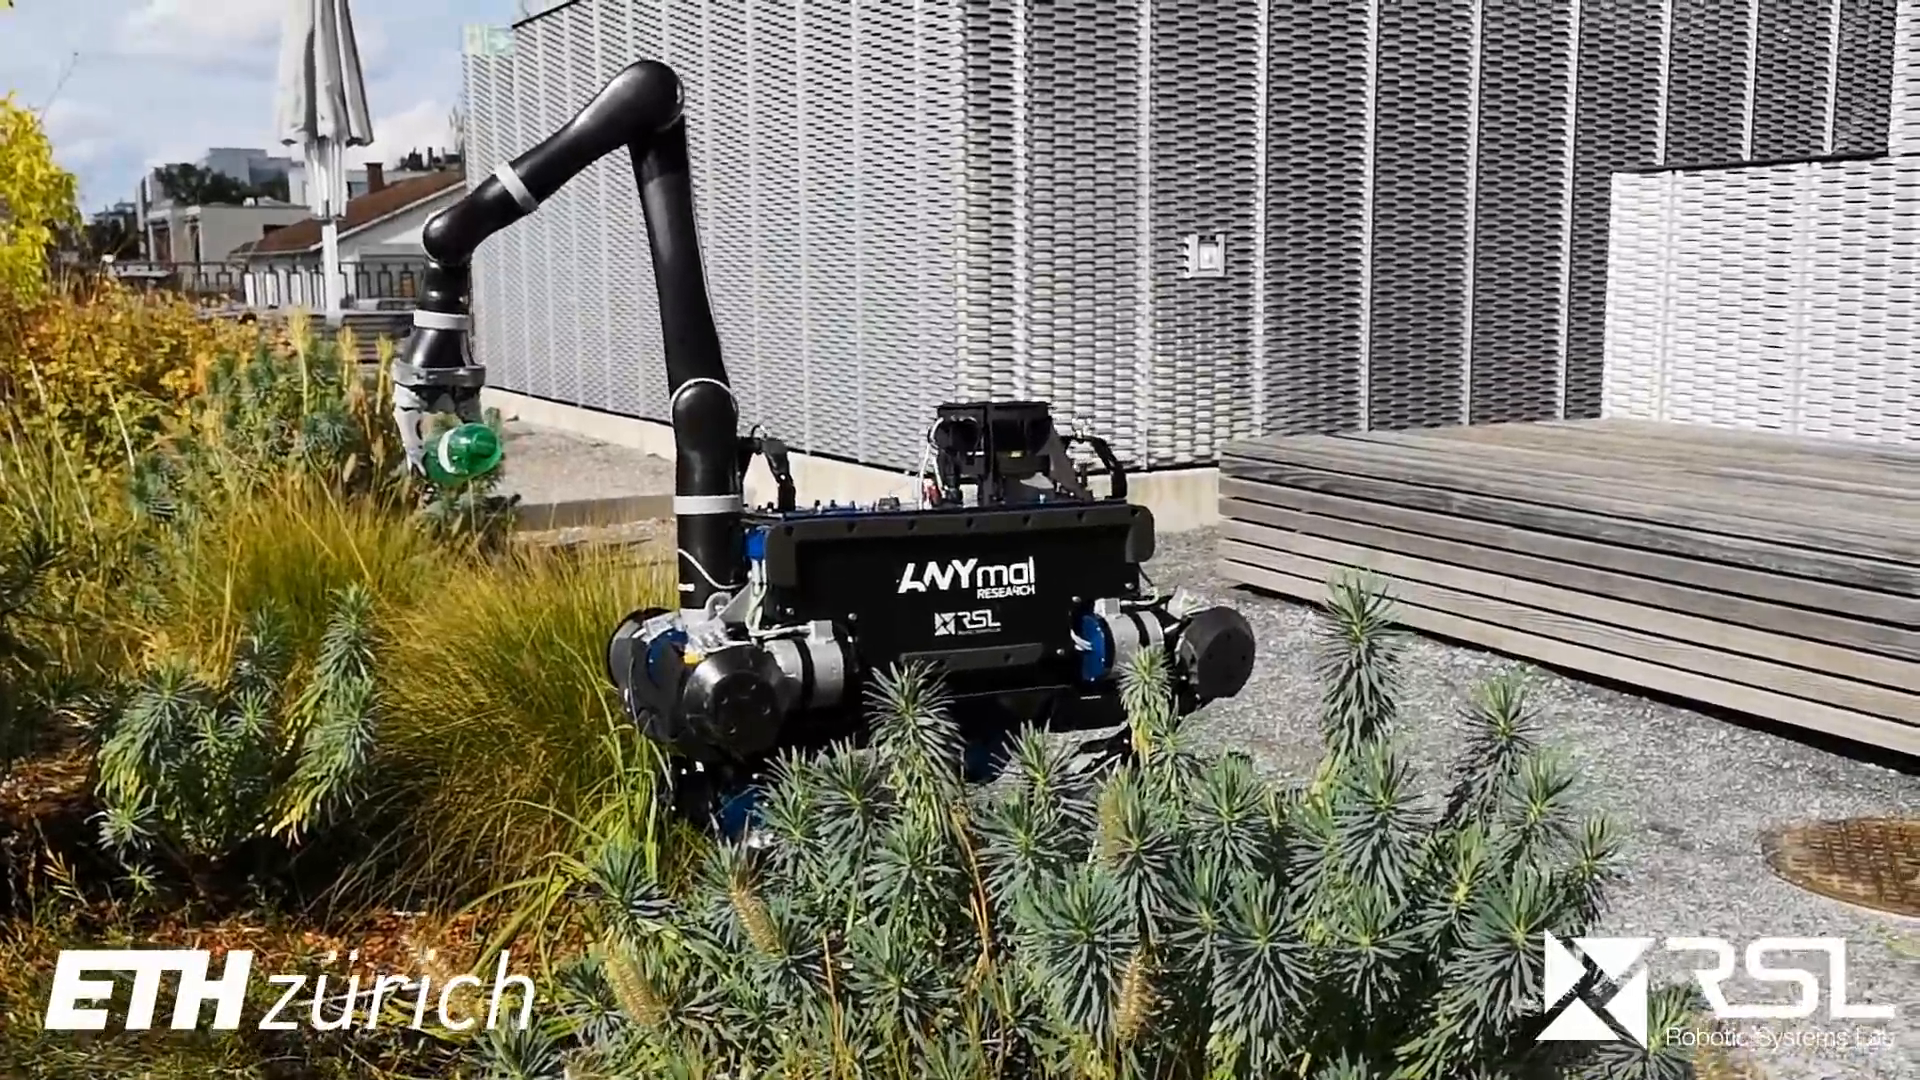
\includegraphics[height=0.5\textwidth]{proposal/alma.png}
    %最终文档中希望显示的图片标题
    \caption{ALMA系统控制框图}
    %用于文内引用的标签
    \label{Fig.1.3}
\end{figure}


在2021年,ETH提出了一种新的基于MPC的全身规划框架\cite{sleiman2021unified}。
该框架通过构建一个多接触最优控制问题,将动态步态运动与操作任务统一起来。
在该框架中,其将通用的机械臂的操作任务建模为一个切换系统,引入了相应约束,
使得在该模型中可以编码任意预定义的步态序列或操作时间表。同时,
该框架将机器人的质心动力学
方程与被操作物体的动力学方程结合,使得机器人能够在相同的代价函数中描述高层次
任务。他们使用该控制框架完成了一系列实验包括开门,推拉重物以及身体与机械臂
的配合动作。基于该框架,在2023年,ETH将轨迹优化与基于采样的图搜索和路径规划结
合\cite{sleiman2023versatile},使得四足机械臂在无人工引导的前提下,
展现了多种操作与运动技巧。该系统框架图如图\ref{Fig.1.4}所示。这类基于M
PC的控制方法可以实现精确的控制,可是面对动态且复杂的环境,控制缺乏鲁棒性。
同时在上述方法中,控制系统往往由多个串联独立的模块组成,每个模块需要单独调试,
整体控制系统十分复杂,并且需要繁琐精细的建模与优化过程\cite{hwangbo2019learning}。
%H为当前位置,!htb为忽略美学标准,htbp为浮动图形
\begin{figure}[H]
    %图片居中
    \centering
    %插入图片,[]中设置图片大小,{}中是图片文件名
    \includegraphics[width=0.88\textwidth]{proposal/mpc_versatile.png}
    %最终文档中希望显示的图片标题
    \caption{将图搜索算法引入MPC系统设计之中,使得机器人能够展示多种运动操作技巧}
    %用于文内引用的标签
    \label{Fig.1.4}
\end{figure}

近些年,强化学习逐渐应用在四足机械臂上。2022年Yuntao等人将基于DRL的四足运动
控制器与基于MPC的机械臂控制器结合起来\cite{ma2022combining},其训练与部署流程图
如图\ref{Fig.1.5}。在此工作中,
机械臂的操作过程被认为是对四足机器人的一种扰动。
为了让四足运动控制器抵抗这种扰动,在仿真训练时,引入干
扰力生成器对四足机器人施加扰动序列,并将该序列引入到观测之中。通过这种方法,
DRL运动控制能够有效的抵抗机械臂的运动扰动。这种方法结合了DRL与MPC,
能够让机械臂精确的追踪参考轨迹。但是这种方法将机械臂与四足机器人视为两个独立
的系统,意味着两者无法产生任何的配合行为。这限制了四足机器人的应用,例如,由于
没有配合行为,四足机械臂无法抓取位于地面上或者处于高处的物体。
%H为当前位置,!htb为忽略美学标准,htbp为浮动图形
\begin{figure}[H]
    %图片居中
    \centering
    %插入图片,[]中设置图片大小,{}中是图片文件名
    \includegraphics[width=0.84\textwidth]{proposal/seperate_control.png}
    %最终文档中希望显示的图片标题
    \caption{基于DRL的运动控制与基于MPC的机械臂控制相结合}
    %用于文内引用的标签
    \label{Fig.1.5}
\end{figure}

DRL方法需要精心设计奖励函数,而对于足式机械臂而言,机械臂的位姿追踪目标与四足
机器人的速度追踪目标相互耦合,有时还相互矛盾。例如,机械臂在运动过程中会对身体
产生很大的扰动,从而影响四足的速度追踪任务。而四足机器人在运动过程中,也会影响
机械臂的位姿追踪。这种相互矛盾的目标使得强化学习奖励设计十分负责,需要耗费大量
工程实践。在同时优化这两个目标时,强化学习方法往往陷入局部最优解。为解决这种缺
陷,Zipeng等人提出了混合优势方法与在线正则方法\cite{fu2023deep},
该方法首次使用DRL方法构建了四足机械臂的统一
的全身控制器,整体系统框架图如图\ref{Fig.1.6}。该方法通过在训练初期分解两个目标奖励,在后期融合两个目标奖励,
成功让策略学习到机械臂与身体动作之间的相互作用。利用该方法,四足机器人能够通过下
伏与上仰等姿势配合机械臂操作,增大了机械臂的操作空间。并且同时,在机械臂操作时,
四足机器人也可以进行运动。基于该方法,Tifanny等人首次使用DRL方法训练了一个四足机械
臂的集成控制器——该控制器能够利用全身关节实现机械臂末端执行器的位姿追踪与力追踪
\cite{portela2024learning}。
%H为当前位置,!htb为忽略美学标准,htbp为浮动图形
\begin{figure}[H]
    %图片居中
    \centering
    %插入图片,[]中设置图片大小,{}中是图片文件名
    \includegraphics[width=0.84\textwidth]{proposal/deep_whole_body_control.png}
    %最终文档中希望显示的图片标题
    \caption{使用强化学习训练足式机械臂统一全身控制器}
    %用于文内引用的标签
    \label{Fig.1.6}
\end{figure}

\section{国内研究现状}
对于四足机械臂这一平台,国内往往采用四足机器人与机械臂独立控制的方案,
这种方法往往采用MPC控制架构,并且机械臂与身体之间完全解耦,
因此两者之间不可能产生合作性的动作,
限制足式机械臂的应用场景。2024年,清华大学与上海AI Lab提出了
RoboDuet四足机械臂强化学习控制框架\cite{pan2024roboduet},如图\ref{Fig.1.7}所示。
该框架需要两个阶段的训练。首先,利用深度强化学习训练一个四足机器人运动控制器,之后,
该运动控制器与一个独立的机械臂控制器同时在四足机械臂平台上进行训练。
这种方法的一个优点是可以利用现有的四足运动控制器降低四足机械臂全身
控制器训练难度。但是这种训练方法更繁琐,并且在第二阶段内,训练过程
更加关注机械臂的位姿追踪任务,会造成四足机器人运动性能的下降。
%H为当前位置,!htb为忽略美学标准,htbp为浮动图形
\begin{figure}[H]
    %图片居中
    \centering
    %插入图片,[]中设置图片大小,{}中是图片文件名
    \includegraphics[width=0.82\textwidth]{proposal/roboduet.png}
    %最终文档中希望显示的图片标题
    \caption{使用分阶段训练的足式机械臂全身控制框架}
    %用于文内引用的标签
    \label{Fig.1.7}
\end{figure}

\chapter{研究内容与技术路线}
\section{研究内容}
综合上述研究现状与现有研究中存在的问题,本次毕业设计将研究在四足机械臂
试验平台上的基于强化学习的全身控制方法。

首先,在面对机械臂轨迹追踪任务与四足机器人速度追踪这两个耦合并且有时
相互矛盾的目标时,目前强化学习架构没有解决这两个目标的联合优化问题,
需要耗费大量人力调节奖励参数,且算法在优化过程中往往陷入局部最优解,
即只关注一个任务而无法做到全身协同配合。其次,基于强化学习的全身控制
方法没有解决机械臂执行精度的问题。由于强化学习采用先在仿真中训练,
再部署到现实生产环境中的技术路线,为弥补仿真环境与真实环境的偏差,
需要在仿真训练中是引入域随机化策略。这种策略能够显著的提高控制器的鲁棒性
但是会损害机械臂的执行精度。最后足式机械臂广泛的应用场景要求全身控制器
需要掌握多种技能,至少,四足机械臂实验平台能够穿越各种复杂地形,并且能够
完成多种操作任务。
\section{技术路线}
基于上述问题,准备采取技术路线如图\ref{Fig.2.1}。第一点是引入显式的运动学模型扩充观测
变量,同时设计相应奖励函数指导强化学习学习过程。由于显式运动学模型的存在,
在给定命令时,我们就可以获得四足机械臂期望关节状态,这种期望的关节状态变
量能够有效的扩充观测,减轻强化学习的难度。同时,基于该目标状态,
我们可以设计一个收敛到该状态的奖励,该奖励始终为正,意味着算法开始就可
以获得期望状态的可达性。这种学习方法能够降低机械臂位姿追踪任务对四足机器
人速度追踪学习的干扰,使得强化学习能够高效的学习四足机器人与机械臂之间
的配合动作。同时,显式的运动学模型提供了精确的逆运动学解,该解将会直接
被critic与actor获得,在一定程度上可以缓解由于域随机化带来的机械臂执
行精度不佳的问题。

第二点引入基于模型的强化学习方法。基于模型的强化学习(Model-Based Reinforcement
Learning, MBRL)\cite{hafner2019dream, hansen2022temporal}通过学习一个环
境模型,在无需与真实环境进行频繁交互的情况下,借助模型模拟大量虚拟数据。
这种方法相比于无模型强化学习(Model-Free ReinforcementLearning,MFRL)
在数据利用效率上更高。具体来说,MBRL 仅需较少的真实环境数据便能
达到良好的性能。此外,MBRL 能利用环境模型进行前向预测,加速策略优化过程,因此在收敛速
度上显著优于MFRL。

另外,通过引入额外的层次结构,MBRL能将复杂任务分解为多个子任务,并利用模型分别优化这
些子任务,从而显著降低学习的复杂度,提高整体任务解决的效率。Hansen等人也指出,
通过学习通用的世界模型,策略可以同时学习和执行多种技能\cite{hansen2023td}。
基于以上优势,MBRL相较于MFRL更加适合解决足式机器人的全身优化问题。

第三点使探索足式机械臂多技能融合的方法。在深度学习中,混合专家模型(Mixture of
Experts, MoE)常常用来扩展深度学习模型的推理能力,MoE独特的网络结构意味着其适合
同时学习多种技能。例如Hoeller等人\cite{hoeller2024anymal}使用了与MoE中门控网络相似的结构,
实现了ANYmal四足机器人的多技能融合,使得机器人能够在结构化的地形中进行跑酷。
目前足式机械臂的技能融合依然在起步探索阶段。

%H为当前位置,!htb为忽略美学标准,htbp为浮动图形
\begin{figure}[H]
    %图片居中
    \centering
    %插入图片,[]中设置图片大小,{}中是图片文件名
    \includegraphics[width=0.84\textwidth]{proposal/road.png}
    %最终文档中希望显示的图片标题
    \caption{研究内容与拟采用的技术路线}
    %用于文内引用的标签
    \label{Fig.2.1}
\end{figure}

\chapter{阶段性进展与进一步研究重点}
\section{研究进展}
目前已经取得了一些阶段性的进展。我们已经实现了通过引入机械臂显式运动学模型指导强化
学习学习过程。目前,我们在仿真引擎之外我们独立设计了一个运动学模块,
该模块可以对机械臂以及四足机器人的腿足进行运动学建模。在训练过程中,
当给定机械臂目标位姿命令时,该运动学模块可以快速地解决逆运动学问题求得机械臂
期望的关节状态位置。该目标状态位置将会传递给critic与actor从而扩展观察状态变量。
扩展的状态变量能让算法提前获得可行解的分布,从而使得机器人快速探索收敛到目标状态。
基于这种方法,我们成功在X20-Z1四足机械臂试验平台上训练出了
一个运动-操作全身控制器。该控制器具有高动态范围,能够抵抗扰动,并且能让我们的足式
机械臂展示大范围的全身配合行为,图\ref{Fig.3.1}展示目前我们控制器能完成了的操作任务。
%H为当前位置,!htb为忽略美学标准,htbp为浮动图形
\begin{figure}[H]
    %图片居中
    \centering
    %插入图片,[]中设置图片大小,{}中是图片文件名
    \includegraphics[width=1.0\textwidth]{proposal/wave.jpg}
    \includegraphics[width=1.0\textwidth]{proposal/grasp.jpg}
    \includegraphics[width=1.0\textwidth]{proposal/pull.jpg}
    %最终文档中希望显示的图片标题
    \caption{全身控制器展现大范围的全身配合运动与多种操作技巧}
    %用于文内引用的标签
    \label{Fig.3.1}
\end{figure}


\section{研究计划与研究重点}
之后的研究计划与研究重点主要如下:首先,解决机械臂与腿足式机器人面对多任物的收敛性
问题,尽量减少扩展到其他足式机械臂上时的繁琐的奖励调节步骤。其次,
解决在足式机械臂在复杂地形行走操作的难以收敛问题。由于足式机械臂需要同时优化
多个任务,并且机器人具有较高的自由度,因此在复杂地形上行走时,强化学习往往只
关注其中一个任务,无法收敛到全局最优点。最后,引入感知信息,解决足式机械臂多技能融合,
提高足式机械臂的执行精度,探索足式机械臂的多应用场景。

%H为当前位置,!htb为忽略美学标准,htbp为浮动图形
\begin{table}[H]
    \zihao{-4}
    \fangsong
    \caption{任务与计划}
    \centering
    {
        \begin{tabularx}{\textwidth}{|X|X|X|} \hline
            \textbf{时间段}                         & \textbf{任务}                 & \textbf{完成进度} \\ \hline
            2023.9.6 \textasciitilde 2024.3.31   & 阅读论文,在仿真中实现全身控制器,验证方法可行性    & 已完成           \\ \hline
            2024.4.1 \textasciitilde 2024.9.30   & 将全身控制系统部署到X20-Z1机器人平台上,撰写论文 & 已完成           \\ \hline
            2024.10.1 \textasciitilde 2024.11.31 & 完成对aliengoZ1足式机械臂的支持        & 正在进行          \\ \hline
            2024.12.01 \textasciitilde 2025.3.20 & 解决全身控制器在复杂地形上的收敛性问题         & 未完成           \\ \hline
            2025.3.21 \textasciitilde 2025.8.31  & 引入视觉感知信息,开发足式机械臂多个技能        & 未完成           \\ \hline
            2025.9.1 \textasciitilde 2025.11.31  & 准备毕业论文撰写                    & 未完成           \\ \hline
            2025.12.01 \textasciitilde 2026.2.28 & 完成毕业论文撰写,准备毕业论文答辩           & 未完成           \\ \hline
        \end{tabularx}
    }
    \label{Table.1}
\end{table}

\cleardoublepage
\begingroup
\linespreadsingle{}
\printbibliography[title={参考文献}]
\endgroup
